% Propietario conservado: /Users/ruben/Documents/New project/output/REVISION_ARGUMENTAL_APERTURAS_CIERRES_20260915/III/spanish_source/manuscrito/sections/05_ciclo_catalan.tex
\section{Décomposition cyclique, quart de tour et moment orienté de Catalan}
\label{iii:iii:sec:catalan}

Le registre dodécaphasique permet de relier la réponse constitutive à
d’autres invariants du transport. Le lien s’établit sur des sous-espaces
et des applications déterminés : le défaut de rang mesure une différence
d’incidence, le déterminant conserve une réponse scalaire et un coefficient
de la résolvante retient l’orientation. La famille de moments qui aboutit
à Catalan intervient à ce dernier niveau.

\subsection{Deux sous-espaces du cycle dodécaphasique}

Dans $\mathbb R^{12}$, soit $C e_j=e_{j+1\bmod12}$ et soient
\begin{equation}
 P_3^{\mathrm{cyc}}=\frac{I+C^3+C^6+C^9}{4},\qquad
 P_4^{\mathrm{cyc}}=\frac{I+C^4+C^8}{3},\qquad
 H_d=\operatorname{Ran}P_d^{\mathrm{cyc}}.
 \label{iii:iii:eq:projectors34}
\end{equation}
Les moyennes sur les sous-groupes cycliques sont des projecteurs orthogonaux.
$H_3$ est formé des suites périodiques de période divisant $3$,
et $H_4$ de celles de période divisant $4$. Leurs dimensions sont $3$ et $4$.
La restriction de $C$ à chaque espace réalise le cycle correspondant.
L’exposant $\mathrm{cyc}$ identifie la moyenne du cycle dodécaphasique :
$P_3^{\mathrm{cyc}}$ est le projecteur sur les suites de période divisant
$3$. Son domaine et son action sont distincts de ceux du projecteur isotypique
tridimensionnel de la réalisation icosaédrique ; la coïncidence des rangs
n’identifie pas les deux opérateurs.

\begin{proposition}[Défaut de rang et réponse déterminantale]
On vérifie
\begin{equation}
 \frac{\operatorname{Tr}(P_3^{\mathrm{cyc}}-P_4^{\mathrm{cyc}})}{12}=-\frac1{12},\qquad
 \frac{\det_{H_3}(I-sC)}{\det_{H_4}(I-sC)}
 =\frac{1-s^3}{1-s^4}=f(s),\quad 0<s<1.
 \label{iii:iii:eq:trace-det}
\end{equation}
\end{proposition}
\begin{proof}
La trace d’un projecteur orthogonal est son rang, de sorte que le numérateur
de la première expression est $3-4$. Le polynôme caractéristique d’un cycle
de longueur $d$ est $t^d-1$ ; son déterminant $\det(I-sC)$ est donc
$1-s^d$. Le quotient produit la seconde identité.
\end{proof}

La substitution $s=q^{30}$ transporte cette représentation vers le quotient
$90/120$. En $s=1$, le mode constant commun s’annule avant de prendre la
limite, qui vaut $3/4$. Cette réalisation de $-1/12$ comme défaut de trace
a un domaine fini explicite. Les réalisations régularisées et
modulaires du même scalaire conservent leurs opérateurs et domaines propres.

\subsection{Représentation fidèle du quart de tour}

Définissons le projecteur antipodal $P_{\rm ant}=(I-C^6)/2$ et
$Q=P_4^{\mathrm{cyc}}P_{\rm ant}$. Ce projecteur agit sur le cycle à douze phases et est
distinct du projecteur constitutif $P_-$ de la section~\ref{iii:iii:sec:constitutiva}.
Les projecteurs $P_4^{\mathrm{cyc}}$ et $P_{\rm ant}$ commutent et
$Q$ est de rang $2$. Dans son image, on fixe la base orthonormée
\begin{equation}
 u=\frac1{\sqrt6}(1,0,-1,0,1,0,-1,0,1,0,-1,0)^{\mathsf T},
 \qquad v=Cu.
 \label{iii:iii:eq:uv}
\end{equation}
On vérifie composante par composante que $Cu=v$ et $Cv=-u$. Par conséquent,
l’isométrie $W(a,b)=au+bv$ satisfait
\begin{equation}
 CW=WJ,\qquad
 J=\begin{pmatrix}0&-1\\1&0\end{pmatrix},\qquad J^2=-I.
 \label{iii:iii:eq:quarter-intertwiner}
\end{equation}
La structure complexe du plan est réalisée par l’action effective du
cycle. Le signe dépend de l’orientation fixée : dans la même base,
$C^3W=-WJ$. Cette précision permet de composer le plan avec le lecteur orienté.

\subsection{Résolvante et profondeur illimitée}

Comme $C^2=-I$ sur $\operatorname{Ran}Q$, pour $0\leq s<1$, on a
\begin{equation}
 (I-sC)^{-1}\big|_{\operatorname{Ran}Q}=\frac{I+sC}{1+s^2},
 \qquad k_4(s):=\langle v,(I-sC)^{-1}u\rangle=\frac{s}{1+s^2}.
 \label{iii:iii:eq:resolvent}
\end{equation}
La suite $\langle v,C^nu\rangle$ est $0,1,0,-1,\ldots$. Le lecteur
de profondeur conserve ce caractère au moyen du moment
\begin{equation}
 \mathcal C_2(s)=\sum_{k\geq0}\frac{(-1)^ks^{2k+1}}{(2k+1)^2},
 \qquad 0\leq s\leq1.
 \label{iii:iii:eq:c2}
\end{equation}
La série converge absolument et uniformément sur cet intervalle par
comparaison avec $\sum(2k+1)^{-2}$. Pour $0<s<1$, les séries dérivées
convergent uniformément sur chaque intervalle compact intérieur. Avec
$\mathcal D=s\,d/ds$, on obtient
\begin{equation}
 \mathcal D^2\mathcal C_2(s)=k_4(s),\qquad
 \mathcal C_2(s)=\int_0^s\frac{dt}{t}\int_0^t\frac{d\xi}{\xi}\,k_4(\xi).
 \label{iii:iii:eq:c2-integral}
\end{equation}
Les conditions $\mathcal C_2(0)=0$ et
$\lim_{s\downarrow0}\mathcal D\mathcal C_2(s)=0$ fixent les deux constantes
d’intégration. En effet, la différence de deux solutions de
$\mathcal D^2F=k_4$ a la forme $a\log s+b$ ; la seconde condition
annule $a$ et la première annule $b$.
La convergence uniforme permet d’évaluer l’extrémité $s=1$ : le résultat est
le moment de Catalan. La représentation finie du caractère conserve son
orientation ; l’indice de profondeur reste illimité.

\subsection{Composition avec la réponse constitutive}

\begin{theorem}[Relation différentielle constitutive]
Pour $0<s<1$, avec l’orientation de \eqref{iii:iii:eq:uv},
\begin{equation}
 f(s)=\frac{1+s+s^2}{s(1+s)}\,\mathcal D^2\mathcal C_2(s).
 \label{iii:iii:eq:catalan-vacuum}
\end{equation}
\end{theorem}
\begin{proof}
Substituer \eqref{iii:iii:eq:resolvent} dans \eqref{iii:iii:eq:c2-integral} et utiliser
$(1+s)(1+s^2)=1+s+s^2+s^3$ donne l’identité. Tous les dénominateurs sont
positifs sur le domaine. L’entrelaceur \eqref{iii:iii:eq:quarter-intertwiner}
identifie le coefficient opératoriel utilisé avant son évaluation.
\end{proof}

En évaluant $s_\pm=q_\pm^{30}$, la même famille produit les deux réponses
de canal de \eqref{iii:iii:eq:rchannels}. La limite de Catalan, le défaut de
trace et les valeurs propres constitutives conservent leurs fonctions différentes
au sein de cette composition. L’inversion du cycle avec les marques $u,v$
fixes change le signe de $k_4$ et conserve le déterminant $1+s^2$.
On identifie ainsi une information d’orientation que le déterminant
seul ne distingue pas.

Le développement de Pell utilise une évaluation particulière de cette famille,
avec $\rho=2-\sqrt3$ et $\rho^{-1}=2+\sqrt3$. Sa preuve est conservée comme
unité d’intégration propre ; la définition angulaire de $q_\pm$ reste
indépendante d’une éventuelle identification de $s_\pm$ à $\rho$.

La figure~\ref{iii:iii:fig:respuesta-momento-pell} représente la relation entre
la réponse rationnelle et le noyau orienté avant l’intégration. La section
de Pell satisfait $\rho+\rho^{-1}=4$, donc
$k_4(\rho)=(\rho+\rho^{-1})^{-1}=1/4$. Les deux valeurs constitutives
s’obtiennent, en revanche, en évaluant $f$ aux arguments $s_\pm$ déjà
construits. Le tracé inclut les prolongements continus des deux
fonctions à $[0,1]$ ; le domaine d’inversion constitutive reste
l’intervalle ouvert $(0,1)$.

\begin{figure}[htbp]
\centering
\begin{tikzpicture}[x=10cm,y=4.6cm,>=stealth]
 \pgfmathsetmacro{\pellrho}{2-sqrt(3)}
 \pgfmathsetmacro{\fpell}{(1+\pellrho+\pellrho^2)/(1+\pellrho+\pellrho^2+\pellrho^3)}
 \draw[gray!35,thin] (0,0.25)--(1,0.25);
 \draw[gray!35,thin] (0,0.5)--(1,0.5);
 \draw[gray!35,thin] (0,0.75)--(1,0.75);
 \draw[gray!35,thin] (0,1)--(1,1);
 \draw[->] (0,0)--(1.04,0) node[right] {$s$};
 \draw[->] (0,0)--(0,1.1) node[above] {valeur adimensionnelle};
 \foreach \xx/\lab in {0/0,0.5/{1/2},1/1}{
  \draw (\xx,0)--(\xx,-0.015) node[below] {$\lab$};
 }
 \foreach \yy/\lab in {0.25/{1/4},0.5/{1/2},0.75/{3/4},1/1}{
  \draw (0,\yy)--(-0.008,\yy) node[left] {$\lab$};
 }
 \draw[gray!70,densely dashed] (\pellrho,0)--(\pellrho,1.035);
 \node[below,align=center,font=\small] at (\pellrho,-0.015)
  {$\rho$\\[-1pt]$2-\sqrt3$};
 \draw[black,very thick,domain=0:1,samples=121,smooth]
  plot (\x,{(1+\x+\x^2)/(1+\x+\x^2+\x^3)});
 \draw[blue!65!black,thick,dashed,domain=0:1,samples=121,smooth]
  plot (\x,{\x/(1+\x^2)});
 \fill[black] (\pellrho,\fpell) circle[radius=1.7pt];
 \fill[blue!65!black] (\pellrho,0.25) circle[radius=1.7pt];
 \node[anchor=south west,font=\small,fill=white,inner sep=2pt] at (0.51,0.94)
  {$f(s)=\dfrac{1+s+s^2}{1+s+s^2+s^3}$};
 \node[anchor=south west,text=blue!65!black,font=\small] at (0.57,0.55)
  {$k_4(s)=\dfrac{s}{1+s^2}$};
 \node[anchor=north west,font=\small,fill=white,inner sep=2pt]
  at (0.30,0.225) {$k_4(\rho)=1/4$};
\end{tikzpicture}
\caption{Réponse constitutive et noyau du moment orienté. La courbe
en trait continu est $f$ et celle en tirets est
$k_4=\mathcal D^2\mathcal C_2$ ; toutes deux sont reliées au moyen de
\eqref{iii:iii:eq:catalan-vacuum}. La droite verticale marque la section de Pell,
sans l’identifier aux arguments constitutifs $s_+$ ou $s_-$.}
\label{iii:iii:fig:respuesta-momento-pell}
\end{figure}
